%%%%%%%%%%%%%%%%%%%%%%%%%%%%%%%%%%%%%%%%%
% a0poster Landscape Poster
% LaTeX Template
% Version 1.0 (22/06/13)
%
% The a0poster class was created by:
% Gerlinde Kettl and Matthias Weiser (tex@kettl.de)
% 
% This template has been downloaded from:
% http://www.LaTeXTemplates.com
%
% License:
% CC BY-NC-SA 3.0 (http://creativecommons.org/licenses/by-nc-sa/3.0/)
%
%%%%%%%%%%%%%%%%%%%%%%%%%%%%%%%%%%%%%%%%%

%----------------------------------------------------------------------------------------
%	PACKAGES AND OTHER DOCUMENT CONFIGURATIONS
%----------------------------------------------------------------------------------------

\documentclass[a0,landscape]{a0poster}

\usepackage{multicol} % This is so we can have multiple columns of text side-by-side
\columnsep=100pt % This is the amount of white space between the columns in the poster
\columnseprule=3pt % This is the thickness of the black line between the columns in the poster

\usepackage[svgnames]{xcolor} % Specify colors by their 'svgnames', for a full list of all colors available see here: http://www.latextemplates.com/svgnames-colors

\usepackage{times} % Use the times font
%\usepackage{palatino} % Uncomment to use the Palatino font

\usepackage{graphicx} % Required for including images
\graphicspath{{figures/}} % Location of the graphics files
\usepackage{booktabs} % Top and bottom rules for table
\usepackage[font=small,labelfont=bf]{caption} % Required for specifying captions to tables and figures
\usepackage{amsfonts, amsmath, amsthm, amssymb} % For math fonts, symbols and environments
\usepackage{wrapfig} % Allows wrapping text around tables and figures

\begin{document}

%----------------------------------------------------------------------------------------
%	POSTER HEADER 
%----------------------------------------------------------------------------------------

% The header is divided into three boxes:
% The first is 55% wide and houses the title, subtitle, names and university/organization
% The second is 25% wide and houses contact information
% The third is 19% wide and houses a logo for your university/organization or a photo of you
% The widths of these boxes can be easily edited to accommodate your content as you see fit

\begin{minipage}[b]{0.55\linewidth}
\veryHuge \color{NavyBlue} \textbf{Recidivism of criminal offenders} \color{Black}\\ % Title
\Huge\textit{A machine-learning approach to justice}\\[1cm] % Subtitle
\huge \textbf{Estienne Granet \& Victor Lei}\\ % Author(s)
\huge Harvard University\\ % University/organization
\end{minipage}


\vspace{1cm} % A bit of extra whitespace between the header and poster content

%----------------------------------------------------------------------------------------

\begin{multicols}{4} % This is how many columns your poster will be broken into, a poster with many figures may benefit from less columns whereas a text-heavy poster benefits from more

%----------------------------------------------------------------------------------------
%	ABSTRACT
%----------------------------------------------------------------------------------------

\color{Navy} % Navy color for the abstract

\begin{abstract}

Recidivism of criminal offenders is a difficult topic in criminal justice. If we view the justice system as serving an important rehabilitatory purpose, then recidivism represents indicators for potential improvement in the correctional system. Using a public data-set on recidivism, we build off of prior work that used both traditional techniques, and machine learning techniques to find the probability of a criminal offender re-offending in the near future given his or her background, as well as the amount of time served. From this probability, we derive the optimal sentence given an individual. Our approach employs two classification methods in an attempt to improve accuracy:

\begin{itemize}
\item Random Forests
\item Neural Networks
\end{itemize}

\end{abstract}

%----------------------------------------------------------------------------------------
%	INTRODUCTION
%----------------------------------------------------------------------------------------

\color{SaddleBrown} % SaddleBrown color for the introduction

\section*{Introduction}
Our goal is to develop a model that accounts for the offender's background and both predicts the probability of recidivism, and computes the optimal sentence. We define the optimal sentence as the sentence that minimizes the probability of recidivism given a set of constraints like making sure life imprisonment does not become the default answer. In particular, we would like to:
\begin{enumerate}
\item derive a predictor$ P$ for the probability of recidivism. The predictor would be a function that takes an individual's background, the nature of their offense and the sentence as inputs, and returns the probability of recidivism as an output; and
\item find the optimal sentence for a given individual with a set of constraints.
$$ \text{argmin}_{\text{sentence}} P(\text{sentence}, \text{others}) $$
under constraints $\text{sentence} \leq \text{threshold}(k)$ where $k$ is the offense committed 
\end{enumerate}

We are using an ICPSR dataset which consists of the profiles of 9,327 prisoners released in 1978 and the profiles of 9,549 prisoners released in 1980. Each entry has 19 variables such as gender, age, sentence, and whether recidivism occurred within the follow-up period (around 4 years.)

\color{DarkSlateGray} % DarkSlateGray color for the rest of the content

\section*{Neural network}
Neural networks were discovered some time ago, but lately, they have been experiencing a resurgence in usage. There is likely significant complexity in the interactions between the different variables, so simple models like logistic regression are not going to be as capable of modeling them compared to neural networks. Prior work on this data set has considered the use of neural networks and found them to have good predictive power for recidivism compared to traditional modeling techniques like logistic regression models. We seek to harness the improvements in neural networks that have been made over the last few years in an attempt to improve predictive accuracy. We find that we can achieve a small, but notable improvement in accuracy on unseen data.

As this is a plain binary classifications problem, we use a multi-layer perceptron feedforward neural network with a single hidden layer, bias terms, and the logistic function as the activation function ($f$) for both the hidden and output layers. There is a single output neuron ($\hat{y} \in (0, 1)$) used for classification with a $0.5$ threshold. For some input vector $x$, linear weights $W$, and bias terms $b$:

\[ \hat{y} = f( W_2  f( W_1 x + b_1 ) + b_2 ) \]
\[ E = - y \ln( \hat{y} ) - (1 - y) \ln ( 1 - \hat{y} ) \]

\begin{center}\vspace{1cm}
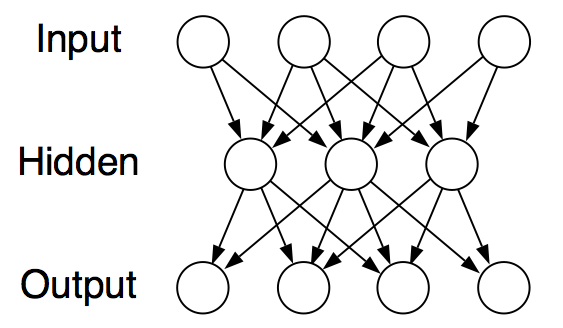
\includegraphics[width=0.8\linewidth]{neural_network}
\captionof{figure}{\color{Green} Feedforward Neural Network\cite{jordan2004introduction}}
\end{center}\vspace{1cm}

Using cross-entropy error ($E$), we can apply backpropagation and optimize the weights and bias terms by stochastic gradient descent using $\frac{\partial E}{\partial W}$, and $\frac{\partial E}{\partial b}$. In order to counteract overfitting, we use an early-stopping heuristic to stop training the model when the validation set performance does not improve for a certain number of epochs.

\begin{wraptable}{l}{12cm} % Left or right alignment is specified in the first bracket, the width of the table is in the second
\begin{tabular}{l l l}
\toprule
\textbf{Dataset} & \textbf{Palocsay et al.} & \textbf{Our results}\\
\midrule
1978 & 69.20\% (39) & 70.69\% (9) \\
1980 & 66.98\% (26) & 68.22\% (5) \\
\bottomrule
\end{tabular}
\captionof{table}{\color{Green} Validation set performance}
\end{wraptable}

After splitting the 1978 dataset and the 1980 dataset into training and validation sets (7:3 ratio) and training the neural network, validation set performance is improved compared to the results from Palocsay et al. The results are also achieved with far fewer nodes in the hidden layer, making it faster to train and likely more generalizable. As the figures below reveal, the neural network starts to quickly overfit as the number of nodes in the hidden layer increases.

\begin{center}\vspace{1cm}
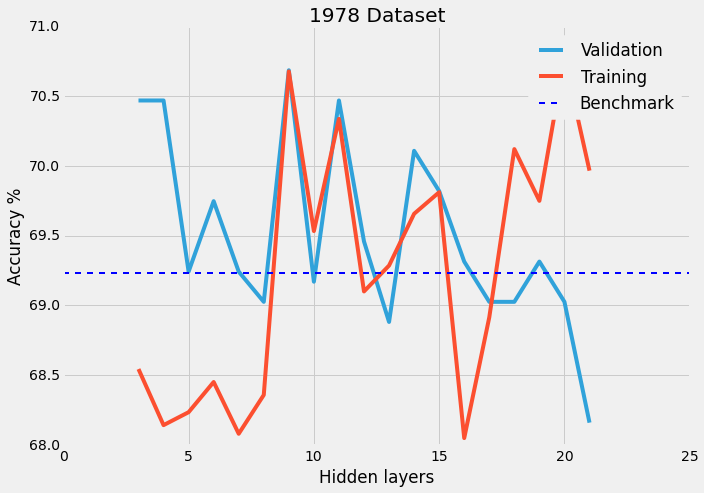
\includegraphics[width=0.9\linewidth]{1978}
\captionof{figure}{\color{Green} 1978 Dataset}
\end{center}\vspace{1cm}

%\begin{center}\vspace{1cm}
%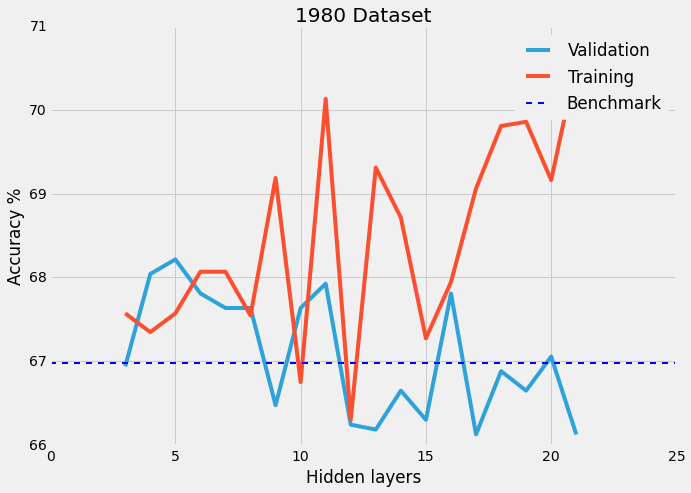
\includegraphics[width=0.9\linewidth]{1980}
%\captionof{figure}{\color{Green} 1980 Dataset}
%\end{center}\vspace{1cm}

\section*{Random Forest}


Phasellus imperdiet, tortor vitae congue bibendum, felis enim sagittis lorem, et volutpat ante orci sagittis mi. Morbi rutrum laoreet semper. Morbi accumsan enim nec tortor consectetur non commodo nisi sollicitudin. Proin sollicitudin. Pellentesque eget orci eros. Fusce ultricies, tellus et pellentesque fringilla, ante massa luctus libero, quis tristique purus urna nec nibh.

Nulla ut porttitor enim. Suspendisse venenatis dui eget eros gravida tempor. Mauris feugiat elit et augue placerat ultrices. Morbi accumsan enim nec tortor consectetur non commodo. Pellentesque condimentum dui. Etiam sagittis purus non tellus tempor volutpat. Donec et dui non massa tristique adipiscing. Quisque vestibulum eros eu. Phasellus imperdiet, tortor vitae congue bibendum, felis enim sagittis lorem, et volutpat ante orci sagittis mi. Morbi rutrum laoreet semper. Morbi accumsan enim nec tortor consectetur non commodo nisi sollicitudin.


\begin{center}\vspace{1cm}
\begin{tabular}{l l l l}
\toprule
\textbf{Treatments} & \textbf{Response 1} & \textbf{Response 2} \\
\midrule
Treatment 1 & 0.0003262 & 0.562 \\
Treatment 2 & 0.0015681 & 0.910 \\
Treatment 3 & 0.0009271 & 0.296 \\
\bottomrule
\end{tabular}
\captionof{table}{\color{Green} Table caption}
\end{center}\vspace{1cm}

Vivamus sed nibh ac metus tristique tristique a vitae ante. Sed lobortis mi ut arcu fringilla et adipiscing ligula rutrum. Aenean turpis velit, placerat eget tincidunt nec, ornare in nisl. In placerat.

\begin{center}\vspace{1cm}

\includegraphics[width=0.8\linewidth]{placeholder}
\captionof{figure}{\color{Green} Figure caption}
\end{center}\vspace{1cm}

%----------------------------------------------------------------------------------------
%	CONCLUSIONS
%----------------------------------------------------------------------------------------

\color{SaddleBrown} % SaddleBrown color for the conclusions to make them stand out

\section*{Conclusions}

\begin{itemize}
\item We improve upon the existing work done by Palocsay et al. on this data set by achieving a higher validation set accuracy using fewer nodes in the hidden layer.
\end{itemize}

\color{DarkSlateGray} % Set the color back to DarkSlateGray for the rest of the content

%----------------------------------------------------------------------------------------
%	FORTHCOMING RESEARCH
%----------------------------------------------------------------------------------------

\section*{Forthcoming Research}

We are still exploring other ways of optimizing the neural network and more advanced regularization strategies like Dropout.

 %----------------------------------------------------------------------------------------
%	REFERENCES
%----------------------------------------------------------------------------------------

\nocite{*} % Print all references regardless of whether they were cited in the poster or not
\bibliographystyle{plain} % Plain referencing style
\bibliography{sample} % Use the example bibliography file sample.bib


\end{multicols}
\end{document}